\documentclass[twocolumn,10pt,a4j]{jsarticle}

\setlength{\topmargin}{-10.4mm} %上端からヘッダーまでの距離
\setlength{\hoffset}{0mm}
\setlength{\voffset}{0mm}
\setlength{\headheight}{0mm} %ヘッダーの高さ
\setlength{\headsep}{0mm} %ヘッダーと本文のスペース
\setlength{\textwidth}{175mm} %文章横 210-35mm
\setlength{\textheight}{267mm} %文章縦 297-30mm
\setlength{\marginparwidth}{20mm}
\setlength{\marginparsep}{0cm}
\setlength{\footskip}{0cm}
\setlength{\columnsep}{20pt} %カラム間のスペース 
\setlength{\oddsidemargin}{-10.4mm} %奇数ページ左サイド余白
\setlength{\evensidemargin}{100mm} %偶数ページ左サイド余白
\newcommand{\figref}[1]{Fig. \ref{#1}} % ラベル参照時の形式を変更した\figrefの定義

\newcommand{\tabref}[1]{Table. \ref{#1}}
\newcommand{\eref}[1]{式(\ref{#1})}

\renewcommand{\figurename}{Fig.} % caption形式の変更
\renewcommand{\tablename}{Table}

\usepackage[dvipdfmx]{graphicx}%画像を挿入するおまじない^^
\usepackage[deluxe]{otf}
\usepackage{svg}

%ボックスで囲むおまじない.
\newsavebox{\MyMiniBox}
\newenvironment{FramedMini}[1]%
 {\begin{lrbox}{\MyMiniBox}%
   \begin{minipage}{#1}}%
   {\end{minipage}%
  \end{lrbox}%
     \fbox{\usebox{\MyMiniBox}}}

\renewcommand\abstractname{}

\begin{document}
\pagestyle{empty}
\renewcommand\abstractname{}

\title{\sffamily 17. Development of Simplified AR Library for Android\\Android向け簡易版ARライブラリの開発}

\author{{\it Yuu~TAMURA}~田村~優\\{\it Supervised~by~Kei~KOGAI}~小飼~敬}
\date{}
\begin{abstract}
 \vspace{-20pt}
 \textbf{Abstract ---} 
 The idea of Augmented Reality (AR) was proposed already several decades ago. However, AR has become much familiar by the appearance of smartphones but it is hard to say that AR has become widespread around the world. Although there are various causes, I thought that one of that is ``difficult to develop them''. So I thought that I could assist the first step of AR development by making a Library for those who learn AR for the first time.
\end{abstract}

\maketitle

\section{はじめに}%研究のきっかけとか.
 2016年,「VR元年」と呼ばれたこの年は,VRの発展が目覚ましく世間の認知度も以前に比べて格段に上がった.VR,すなわち仮想現実感は視界を完全に遮って完全な仮想空間の視界を提供するが,似たようなものにAR,拡張現実感がある.拡張現実感は仮想現実感と違い視界を完全には遮らず,実際の視界に新たな情報を組み込みこんだような視界を提供する技術である.視界を完全に遮るため屋外での使用に限界がある仮想現実感に比べ,拡張現実感は視界を遮らないために幅広い使い方が可能であり,今後様々なシーンで拡張現実感が活用されるだろうと予想できる.しかしこのような予想は数十年前からされており,実現に向けて様々な研究が行われてきた今でも世界に拡張現実感が浸透しているかと言われると肯定はできないだろう.拡張現実感を一気に身近な物にしたスマートフォンでさえ火付け役になれなかった.このような実態を考えた時,まず挙げられる原因は「開発の難しさ」であると考えた.拡張現実感を実装するためには膨大な知識と時間が必要であり,それが開発者を拡張現実感から遠のかせていたと考えられる.しかし近年ARToolKit~\cite{ARToolKit}などのライブラリが公開され以前に比べ開発が容易になっている.そこで今回,ARアプリケーションの開発の最初のハードルをできるだけ下げようとARToolKitをさらに簡単に使用できるように改良することにした.デバイスは先ほど述べたように拡張現実感との相性がとても良く,開発者が多いAndroidを選択した.

\section{現状}%スタート地点

\subsection{開発環境}
近年のAndroid開発環境は以前まで使用されていたEclipseからAndroidStudio~\cite{AndroidStudio}へと移り変わっている.

\subsection{ライブラリ}
主に以下のライブラリが提供されている.
\begin{itemize}
 \item ARToolKit
       \begin{itemize}
	\item OS X, Windows, Linux, iOS, Androidなど,様々なプラットフォームで提供されている.\\
       \end{itemize}
 \item NyARToolKit
       \begin{itemize}
	\item Java, C\#, ActionScript, Processing, Unitiy, C++, Android, Windowsなど,様々なプラットフォームで提供されている.
       \end{itemize}
 \item AndAR
       \begin{itemize}
	\item 近年登場したAndroid専用のARライブラリ.プラットフォーム上でのARを最小限の労力で実現することを目的に作成されている.
       \end{itemize}
\end{itemize}

%\vspace{-15pt}
\section{設計}%何を使ってどんなものを作るか
%\vspace{-5pt}
\subsection{環境}
現状を踏まえて,以下の環境で開発することにした.

\begin{itemize}
 \item OS : Mac OS X Yosemite
       \begin{itemize}
	\item 動作の安定性,今後iOS版の開発をする可能性などを考慮し,Mac miniを使用した.
       \end{itemize}
 \item 開発環境 : AndroidStudio 2.2.2
       \begin{itemize}
	\item 近年の開発環境の遷移を踏まえて,これからのスタンダードとなるであろうAndroidStudioを選択した.
       \end{itemize}
 \item 使用ライブラリ : ARToolKit version: 5.3.1
       \begin{itemize}
	\item Androidの最新versionに対応している他,様々なプラットフォームに対応しているため今後の展開を考えてARToolKitを選択した.
       \end{itemize}
 \item 実行端末 : Nexus9
       \begin{itemize}
	\item Android 7.0が動作するNexus9をARアプリケーションの実行端末として使用した.
       \end{itemize}
\end{itemize}

%\vspace{-5pt}
\subsection{コンセプト}
以下の特徴を持つライブラリを作成する.
\begin{itemize}
 \item 関数名や変数名などをできるだけ分かり易い単語で記述する.
 \item クラスをMain,Setup,ARの三つで構成し,各クラスの役割を明瞭化する.
 \item 拡張し易い構成にする.
 \item MainActivity\footnote{Androidアプリケーションを実行した時,一番最初に実行されるメソッド}はできるだけ最小限にする
\end{itemize}

%画像(PDF)を挿入
%\vspace{-2zh}
\begin{figure}[tb]
 \centering
 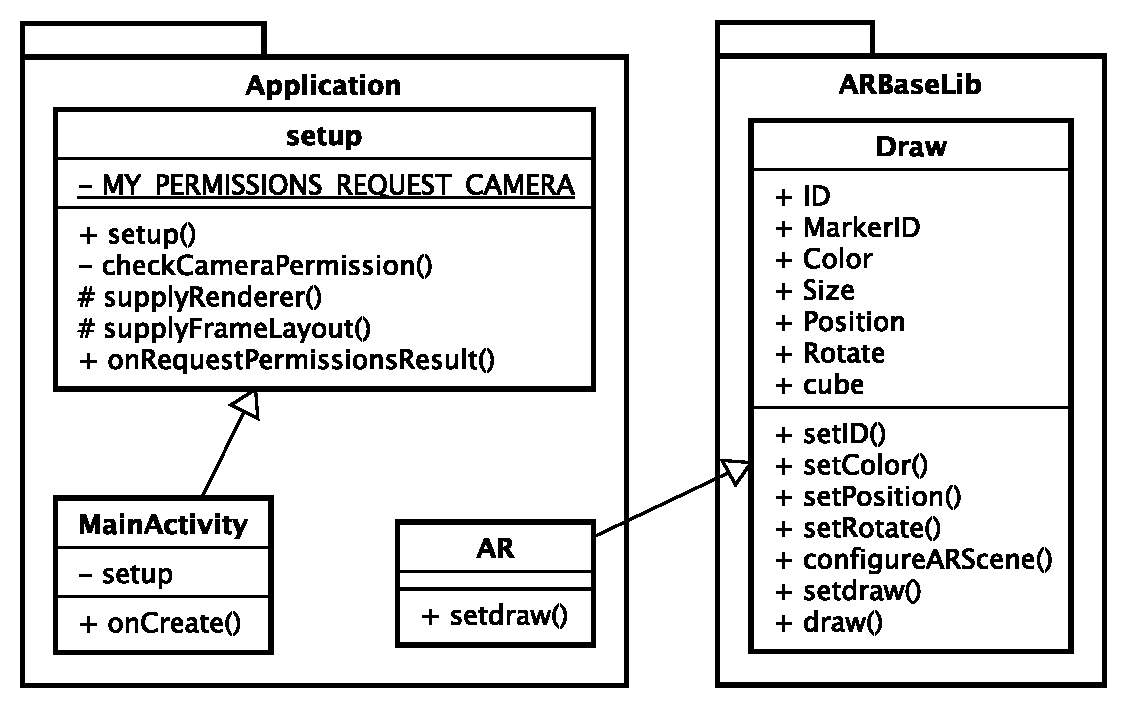
\includegraphics[width=8cm]{fig/class.pdf}
 \caption{Class diagram}
 \label{fig:class}
\end{figure}
%\vspace{-3zh}

\section{実装}%何を作ったか
本研究で実装したクラスのクラス図をFig.\ref{fig:class}に示す.

\subsection{Appモジュール}	

\subsubsection{MainActivity}
MainActiviyクラスは親クラスを変更し,Setupを呼び出すだけとなっている.

\subsubsection{Setup}
Setupクラスは提供されるライブラリ内ではできない各種設定をするクラスである.難しい設定などを全て集めている為,ライブラリと共に提供されるクラスである.使用者は提供されたSetupクラスをMainActivityと同じパッケージに入れるだけで実装が完了する.

\subsubsection{AR}
ARクラスは実際にARで表示したい物体の設定をするクラスである.簡易化を図る為,表示できるのはBoxのみである.Boxの大きさ,色,位置,角度,対応するARマーカを登録するクラスである.

\subsection{ライブラリ}
\subsubsection{Draw}
Drawクラス内にARマーカの検出,及びBoxの表示をする処理が入っている.複数のマーカに反応させる場合,ここの処理を変更しないといけない.

\subsubsection{ARSimpleApplication}
ARToolKitライブラリでAppモジュールに追加しないといけないクラスだったが,処理の明瞭化を図る為ライブラリ内に移動した.


\section{評価}%作ったものの評価
\subsection{達成項目}
\begin{itemize}
 \item 関数名や変数名は分かりやすくなったと言える.
 \item クラスをコンセプトの通りに構成し明瞭化されたと言える.
 \item 目標の一つであるMainActivityの最小限化は達成したと言える.
\end{itemize}
		
\subsection{未達成項目}
\begin{itemize}
 \item 拡張性は十分でなく,複数のマーカに反応させる為にはライブラリ内を変更しないといけない.
\end{itemize}
		
拡張性に関してはライブラリ内を変更しないといけない為にAndroidの知識が必要である.Androidの開発をした事がある人であれば,拡張は難しくは無いだろう.しかし今回は「簡易化」が目的なので未達成と判断した.
		

\section{考察}%考察という名の反省
コンセプトの一つとして「拡張し易い構造」があったが,現時点では拡張性は低く達成できたとは言えない.しかし,Boxを表示する事に限って言えばAndroid開発をした事が無い人でも以前より簡単にARを体験する事ができるようになったと言える.今後,このライブラリを更に改良して拡張性を持たせる事ができれば,AndroidでARを体験する為のライブラリとして有用になると考える.また,表示した後の操作をサポートすることができれば更に可能性が広がるだろう.


\section{おわりに}%まとめ
 Androidアプリケーション開発初学者でも,比較的簡単にARを体験する事ができるようになったと考える.ディスプレイを見ながらカメラを動かすのではなく,カメラの視点と自分の視点がほぼ同じで直感的な操作ができる点でAndroidはとても有用であり,今後の発展も望めるだろう.しかし今のままではただ箱を表示するだけの機能しかなく,多彩な処理をしたい場合には向いて無い.今後は3Dオブジェクトの表示,Raspberry PiなどARアプリケーションの出力先としての装置との連携など,更にARの入門用ライブラリとしての十分な機能を実装したい.


%参考文献
\begin{thebibliography}{1}
 \bibitem{ARToolKit}
	 ARToolKit - Android Documentaion\\
	 http://artoolkit.org/documentation/doku.php?id=\\4\_Android:android\_about
 \bibitem{AndroidStudio}
	 Android Developers Site - Android Studio\\
	 https://developer.android.com/studio/intro/index.html
\end{thebibliography}


\end{document}

